% =====================================================================
% DOCUMENTO-MESTRE — Manual Técnico RAG + Recamán (R456)
%
% Arquitetura modular: cada seção vive em um arquivo separado
% (sec_XX_*.tex) e é incluída aqui via \input. Para aprofundar uma
% seção, edite apenas o arquivo correspondente e recompile main.tex.
%
% Compilar:  ./build.sh   ou   make
% Classe:    abntex2 (local: publishing/templates/abntex2)
% =====================================================================
\documentclass[
	article,
	11pt,
	oneside,
	a4paper,
	english,
	brazil,
	sumario=tradicional
	]{abntex2}

% --- Pacotes fundamentais ---
\usepackage[T1]{fontenc}
\usepackage[utf8]{inputenc}
\usepackage{lmodern}
\usepackage{indentfirst}
\usepackage{microtype}
\usepackage{graphicx}
\usepackage{color}
\usepackage{xcolor}

% --- Matemática e algoritmos ---
\usepackage{amsmath}
\usepackage{amssymb}
\usepackage{algorithm}
\usepackage{algpseudocode}

% --- Tabelas ---
\usepackage{booktabs}
\usepackage{longtable}
\usepackage{tabularx}
\usepackage{array}

% --- Diagramas ---
\usepackage{tikz}
\usetikzlibrary{positioning,arrows.meta,shapes.geometric,calc,fit}

% --- Listagens de código ---
\usepackage{listings}
\lstset{
  basicstyle=\ttfamily\footnotesize,
  frame=single,
  breaklines=true,
  language=Python,
  keywordstyle=\bfseries\color{blue!60!black},
  commentstyle=\color{gray!60!black},
  stringstyle=\color{red!50!black}
}

% --- Enumeração/ambiente ---
\usepackage{enumitem}

% --- Citações ABNT ---
\usepackage[alf]{abntex2cite}
\usepackage[brazilian,hyperpageref]{backref}

% --- Índice remissivo ---
\usepackage{makeidx}
\makeindex

% --- Hiperlinks (abntex2 já carrega hyperref; configuramos opções) ---
\hypersetup{hidelinks=true}
\usepackage{caption}

% ---------------------------------------------------------------
% Infraestrutura didática de profundidade progressiva
% ---------------------------------------------------------------
% Caixa de intuição: traduz um conceito formal em uma analogia acessível.
\newenvironment{intuicao}{%
  \par\medskip\noindent
  \begin{quote}
  \color{blue!55!black}\textbf{\small Caixa de intuição.} \itshape
}{%
  \end{quote}\par\medskip
}

% Caixa de "ponto-chave": sintetiza o que o leitor deve reter ao fim de uma seção.
\newenvironment{pontochave}{%
  \par\medskip\noindent
  \begin{quote}
  \color{black!70}\textbf{\small Ponto-chave.} \normalfont
}{%
  \end{quote}\par\medskip
}

% Marcador de nível de leitura didático:
%   \nivel{0} fundamento/intuição | \nivel{1} aplicação | \nivel{2} rigor formal
\newcommand{\nivel}[1]{%
  \marginpar{\color{gray}\footnotesize N\raisebox{0.1ex}{\scriptsize #1}}%
  {\color{gray!70}\small\textbf{(nível \raisebox{0.1ex}{\scriptsize #1})} }%
}

% ---------------------------------------------------------------
% Configuração da capa
% ---------------------------------------------------------------
\renewcommand{\imprimircapa}{%
  \begin{capa}%
    \center
    \ABNTEXchapterfont\Large\textbf{Ecossistema OpenCode}
    \vspace{0.2cm}
    \ABNTEXchapterfont\large{Núcleo de Documentação Técnica}
    \vspace{1.2cm}

    {\ABNTEXchapterfont\bfseries\large MANUAL TÉCNICO}

    \vspace{0.6cm}
    {\ABNTEXchapterfont\bfseries\LARGE Arquitetura de Recuperação Aumentada por Geração (RAG)}

    \vspace{0.4cm}
    {\ABNTEXchapterfont\large Estado Atual e Proposta de Diversificação Estruturada via Sequência de Recamán}

    \vspace{1.6cm}
    {\large\textbf{Marcelo Claro Laranjeira}}

    \vspace{0.2cm}
    {\small ORCID: \texttt{0000-0001-8996-2887} \quad E-mail: \texttt{marceloclaro@gmail.com}}

    \vspace{1.8cm}
    {\large\textbf{Especificação formal:} SPEC-935-R456}

    \vspace{0.3cm}
    {\large\textbf{Rodada:} R456}

    \vspace{0.3cm}
    {\large\textbf{Data:} 30 de agosto de 2026}

    \vspace{1.5cm}
    {\small Documento técnico confidencial do ecossistema.}

  \end{capa}%
}

% ---------------------------------------------------------------
% Metadados
% ---------------------------------------------------------------
\titulo{Arquitetura de Recuperação Aumentada por Geração (RAG): Estado Atual e Proposta de Diversificação Estruturada via Sequência de Recamán}
\autor{Marcelo Claro Laranjeira}
\local{São Paulo, Brasil}
\data{2026}
\instituicao{Ecossistema OpenCode --- Documentação Técnica}
\orientador{}
\coorientador{}

% =====================================================================
\begin{document}

% --- Capa, folha de rosto, resumo, sumário e listas ---
% =====================================================================
% SEC_00 — Capa, folha de rosto, resumo, sumário e listas
% =====================================================================

% Capa
\imprimircapa

% Folha de rosto
\newpage
\begin{center}
{\large\imprimirtitulo}
\end{center}
\vspace{1cm}
\begin{center}
{\large Autor: \imprimirautor}
\end{center}
\vspace{0.2cm}
\begin{center}
{\small ORCID: \texttt{0000-0001-8996-2887} \quad E-mail: \texttt{marceloclaro@gmail.com}}
\end{center}
\vspace{0.5cm}
\begin{center}
{\normalsize Especificação: SPEC-935-R456 (Rodada R456)}
\end{center}
\vspace{1cm}

\textbf{Resumo:} Este manual documenta a arquitetura de Recuperação Aumentada por
Geração (RAG) do ecossistema, distinguindo rigorosamente o \textbf{estado atual}
(implementado e observável no código-fonte) da \textbf{arquitetura-alvo proposta}
(não implementada) que integra um Diversificador Estruturado baseado na sequência
de Recamán para aumentar a diversidade semântico-estrutural dos resultados
recuperados. O documento parte de um \textbf{problema de pesquisa} formalizado,
que motiva o estudo de diversificação estruturada, e apresenta mapas de
arquitetura, diagramas com legendas, cálculos e especificações técnicas
reproduzíveis, apoiados em referências reais verificadas (DOIs e preprints arXiv).
Foi escrito para uma trilha de leitura de profundidade progressiva --- do leitor
de nível introdutório ao leitor de pós-graduação.

\vspace{0.5cm}
\textbf{Palavras-chave:} RAG; Recuperação de Informação; Recamán; Diversificação;
Geração Aumentada por Recuperação; Arquitetura de Software; Problema de Pesquisa.

\newpage

% ---------------------------------------------------------------
% Sumário
% ---------------------------------------------------------------
\pdfbookmark[0]{\contentsname}{toc}
\tableofcontents*
\clearpage

% Lista de figuras e tabelas (formato banca)
\pdfbookmark[0]{\listfigurename}{lof}
\listoffigures*
\clearpage
\pdfbookmark[0]{\listtablename}{lot}
\listoftables*
\clearpage


% --- Corpo (seções numeradas) ---
% =====================================================================
% SEC_01 — Introdução e Escopo
% =====================================================================

\section*{1. Introdução e Escopo}
\addcontentsline{toc}{section}{1. Introdução e Escopo}

\nivel{0} Este manual tem duas finalidades complementares. A primeira é documentar,
de forma precisa e verificável, a arquitetura de Recuperação Aumentada por
Geração (RAG) tal como \emph{implementada} no ecossistema, referenciando os
módulos reais do código-fonte. A segunda é apresentar uma \textbf{proposta} de
evolução dessa arquitetura: a introdução de um estágio de diversificação
estruturada baseado na sequência matemática de Recamán, que atua sobre o
ranqueamento dos candidatos recuperados.

\begin{intuicao}
Pense no RAG como um assistente de pesquisa que, antes de responder, consulta
uma biblioteca. A qualidade da resposta depende de \emph{quais livros} ele
coloca sobre a mesa. O ponto central deste manual é simples: às vezes a mesa fica
cheia de livros muito parecidos entre si. A \emph{diversificação} tenta resolver
isso, garantindo que os livros representem ângulos diferentes do tema.
\end{intuicao}

\nivel{2} É fundamental registrar uma distinção metodológica que orienta todo o
documento: a arquitetura \emph{atual} é observável e auditável no checkout,
enquanto a arquitetura \emph{pós-Recamán} configura um desenho-alvo
\textbf{proposto}, ainda não implementado. Esta separação entre o que \emph{é} e
o que \emph{poderia ser} sustenta o rigor anti-overclaim do ecossistema
(SDD/TDD): nenhum resultado é apresentado como implementado sem ser observável no
código. Nenhuma alegação de certificação externa, de segurança absoluta ou de
disponibilidade universal de serviços é feita aqui.

\begin{pontochave}
Ao final desta leitura, você deve ser capaz de: (i) distinguir o estado atual da
proposta pós-Recamán; (ii) identificar o problema de pesquisa que motiva a
diversificação; (iii) compreender a intuição por trás do uso da sequência de
Recamán; e (iv) localizar as especificações técnicas e referências que sustentam
cada afirmação.
\end{pontochave}

\subsection*{1.1 Como ler este manual (trilha de profundidade)}

\nivel{0} Este manual foi escrito para ser lido por camadas. Cada seção é
marcada com um \textbf{nível de profundidade} (N0, N1 ou N2) que indica o grau de
formalização exigido:

\begin{center}
\begin{tabularx}{\textwidth}{llX}
\toprule
\textbf{Nível} & \textbf{Tipo de leitor} & \textbf{Em que consiste} \\
\midrule
N0 & Introdutório & Intuição, analogias e motivação; a "história" do problema. \\
N1 & Aplicado & Como os conceitos se materializam em componentes; leitura de
diagramas, tabelas e trechos de código. \\
N2 & Pós-graduação & Formalização matemática, equações, complexidade
assintótica e diálogo com a literatura (referências reais). \\
\bottomrule
\end{tabularx}
\end{center}

\noindent O leitor de nível 0 pode percorrer apenas os parágrafos marcados N0 e
as \emph{Caixas de intuição}. O leitor de nível PhD deve percorrer tudo, incluindo
as equações e as referências. Nenhuma informação é "escondida": a mesma ideia
aparece em várias profundidades, de forma didática, sem sacrificar o rigor da
publicação.

\subsection*{1.2 Estrutura do documento}

O manual está organizado da seguinte forma:

\begin{enumerate}[label=\arabic*.]
  \item \textbf{Introdução e escopo} --- esta seção.
  \item \textbf{Problema de pesquisa e impactos} --- formulação do problema que
        motiva o estudo e seus impactos na ciência e no ecossistema.
  \item \textbf{Fundamentação teórica} --- modelos de ranqueamento, RAG e MMR.
  \item \textbf{Estado atual da arquitetura RAG} --- componentes implementados.
  \item \textbf{Proposta pós-Recamán} --- arquitetura-alvo e diversificador.
  \item \textbf{Cálculos e especificações técnicas} --- equações e métricas.
  \item \textbf{Implementações reproduzíveis} --- pseudocódigo e trechos.
  \item \textbf{Mapas de dados e diagrama operacional} --- visualização.
  \item \textbf{Considerações finais e trabalho futuro}.
\end{enumerate}

\subsection*{1.3 Princípios de rigor}

\nivel{2} Seguindo o protocolo de rigor do ecossistema (SDD/TDD e anti-overclaim),
todo resultado aqui apresentado é ou (i) observável no código, ou (ii)
reproduzível a partir das especificações, ou (iii) claramente rotulado como
proposta. As referências bibliográficas correspondem a fontes reais validadas ---
DOIs de periódicos/conferências e preprints arXiv --- e nenhuma foi fabricada.
A didática nunca substitui a precisão: analogias são sempre acompanhadas da
formalização correspondente.

% =====================================================================
% SEC_02 — Problema de Pesquisa e Impactos
% =====================================================================

\section*{2. Problema de Pesquisa e Impactos}
\addcontentsline{toc}{section}{2. Problema de Pesquisa e Impactos}

\subsection*{2.1 Contextualização do problema}

\nivel{0} Toda investigação nasce de uma insatisfação: algo não funciona tão bem
quanto deveria. Neste manual, a insatisfação é a seguinte: quando um sistema de
recuperação devolve respostas a uma pergunta, ele tende a devolver resultados
\emph{concentrados} --- todos muito parecidos entre si. Isso é útil quando a
pergunta tem uma única resposta certa, mas é um problema quando a pergunta admite
múltiplos ângulos, como numa revisão de literatura ou numa síntese que precisa
cobrir pontos de vista distintos.

\begin{intuicao}
Imagine pedir a um bibliotecário "liste livros sobre mudanças climáticas". Um
sistema comum traria dez livros de física atmosférica. Mas a pergunta que você
realmente tinha era sobre o \emph{impacto econômico} e o \emph{impacto social}
das mudanças climáticas. O bibliotecário "muito relevante demais" perdeu a
\emph{diversidade} que você precisava.
\end{intuicao}

\nivel{2} Do ponto de vista formal, o fenômeno é bem documentado: ranqueadores
lexicais (BM25, Eq.~\ref{eq:bm25}) e densos tendem a concentrar o ranking em um
subespaço semântico homogêneo, privilegiando \emph{relevância individual} em
detrimento de \emph{cobertura} do espaço de interpretações. A literatura de
diversificação, tendo como marco o \emph{Maximal Marginal Relevance} (MMR)
\cite{CarbonellGoldstein1998MMR}, mostra que o equilíbrio entre relevância e
novidade é alcançável, mas frequentemente à custa de parametrizações heurísticas e
de comportamento não determinístico.

\subsection*{2.2 Formulação do problema de pesquisa}

\nivel{2} A partir dessa contextualização, este manual delimita o seguinte
problema de pesquisa, com critérios de auditabilidade:

\begin{quote}
\textbf{Problema de pesquisa (PP).} Como introduzir um estágio de
\textbf{diversificação estruturada} na arquitetura RAG do ecossistema que: (i)
seja \textbf{determinístico} e \textbf{reproduzível} (mesma entrada $\Rightarrow$
mesma saída); (ii) opere \textbf{após} o ranqueamento semântico-estrutural, sem
degradar a relevância primária; e (iii) tenha \textbf{custo assimptótico}
controlável, compatível com pipelines de grande escala?
\end{quote}

Para operacionalizar o problema, derivamos as seguintes \textbf{perguntas de
pesquisa} (RQ):

\begin{enumerate}[label=\textbf{RQ\arabic*.}]
  \item \textbf{RQ1 --- Diversidade.} É possível aumentar a diversidade média do
        conjunto recuperado (Eq.~\ref{eq:diversity}) sem sacrificar a precisão do
        ranqueamento primário?
  \item \textbf{RQ2 --- Determinismo.} A diversificação pode ser tornada
        totalmente determinística e reproduzível, eliminando variações por \emph{seed}
        ou por ordem de execução?
  \item \textbf{RQ3 --- Custo.} Qual é a complexidade assimptótica de tempo e
        memória do estágio de diversificação, e ela é compatível com o pipeline
        existente?
  \item \textbf{RQ4 --- Impacto multiárea.} A diversificação produz benefícios
        observáveis nos fluxos do ecossistema (acadêmico, jurídico, clínico, MIRA)
        que dependem do RAG?
\end{enumerate}

\noindent A \textbf{hipótese central} (H1) é:

\begin{quote}
\textbf{H1.} A sequência de Recamán pode ser usada como \emph{gerador
determinístico de offsets} de diversificação que incrementa a cobertura semântica
do conjunto recuperado com custo $O(K)$ (sobre um ranking indexado de $N$
candidatos), sem exigir retreinamento do modelo de ranqueamento.
\end{quote}

\begin{pontochave}
O problema de pesquisa é, em essência, \emph{determinismo aplicado à
diversificação}: usar uma sequência matemática bem comportada (Recamán) para
garantir que a diversidade seja reproduzível, mensurável e barata.
\end{pontochave}

\subsection*{2.3 Impactos na Ciência}

\nivel{2} O problema descrito conecta-se a fronteiras ativas de pesquisa em
Recuperação de Informação (IR) e Processamento de Linguagem Natural (PLN). Os
impactos potenciais na ciência são:

\begin{enumerate}[label=\arabic*.]
  \item \textbf{Diversificação determinística.} A literatura tradicional de
        diversificação (MMR, Eq.~\ref{eq:mmr}) depende de parâmetros heurísticos
        ($\lambda$) e de medidas de similaridade que introduzem dependência de
        implementação. Uma abordagem determinística baseada em uma sequência
        matemática canônica oferece um \textbf{baseline reproduzível} que pode ser
        comparado de forma justa entre sistemas \cite{CarbonellGoldstein1998MMR}.
  \item \textbf{Conexão entre teoria dos números e IR.} O uso de uma sequência da
        teoria dos números (Recamán), cujas propriedades ainda são objeto de
        investigação \cite{Alekseyev2022RecamanCousins}, abre um diálogo
        interdisciplinar: propriedades combinatórias da sequência podem informar a
        distribuição de offsets de diversidade. Trata-se de uma contribuição
        metodológica (a \emph{ponte} entre dois campos), não de um resultado
        empírico já validado.
  \item \textbf{Rigor metodológico em RAG.} O RAG moderno enfrenta problemas de
        reprodutibilidade (variações por \emph{seed}, ordem de recuperação) e de
        degradação quando a recuperação falha \cite{Yan2024CRAG}; a posição dos
        documentos no contexto impacta a qualidade \cite{Liu2024LostMiddle}. Um
        estágio determinístico de diversificação contribui com uma dimensão
        adicional de reprodutibilidade para avaliações experimentais
        \cite{Ram2023RetrievalAugmented}.
  \item \textbf{Complemento, não substituto.} A proposta não substitui os avanços
        em RAG auto-adaptativo \cite{Jeong2024AdaptiveRAG}, recuperação por grafos
        \cite{Edge2024GraphRAG} nem correção pós-recuperação \cite{Yan2024CRAG};
        ela os \emph{integra} como um estágio de pós-processamento ortogonal,
        preservando a interface dos fluxos consumidores.
\end{enumerate}

\begin{pontochave}
O impacto científico pretendido é \emph{metodológico}: estabelecer uma ponte
reproduzível entre teoria dos números e diversificação de recuperação, que possa
ser avaliada de forma justa e comparável pela comunidade.
\end{pontochave}

\subsection*{2.4 Impactos no Ecossistema OpenCode Ecosystem Core}

\nivel{1} O OpenCode Ecosystem Core opera múltiplos fluxos que consomem RAG como
subsistema transversal. A vantagem potencial da proposta no ecossistema decorre do
fato de que esses fluxos se beneficiam de \emph{cobertura} semântica:

\begin{itemize}
  \item \textbf{Fluxo acadêmico} (revisão de literatura): a diversificação pode
        ampliar o leque de obras e correntes teóricas recuperadas, reduzindo a
        concentração em um único paradigma.
  \item \textbf{Fluxo jurídico} (recuperação normativa): múltiplos dispositivos
        legais e doutrinas podem ser cobertos de forma mais abrangente.
  \item \textbf{Fluxo clínico} (suporte à decisão): a identificação de múltiplos
        ângulos diagnósticos/terapêuticos pode melhorar a revisão de alternativas.
  \item \textbf{Fluxo MIRA} (geração de conteúdo): a síntese multi-perspectiva
        torna o conteúdo gerado mais rico e equilibrado.
\end{itemize}

\nivel{2} É importante registrar, com rigor, o \textbf{limite do impacto}: os
benefícios descritos são \emph{potenciais} e \emph{hipotéticos}, dependentes da
implementação e de validação empírica futura. Este manual \emph{não} afirma que a
diversificação por Recamán já produz tais benefícios no ecossistema --- trata-se
de uma hipótese (H1) e de uma direção de impacto a ser medida nas RQs. A
arquitetura pós-Recamán permanece \textbf{proposta, não implementada}.

\begin{pontochave}
O impacto no ecossistema será \emph{medido}, não presumido: cada benefício
potencial listado acima está vinculado a uma RQ e será validado por métricas
(como a Eq.~\ref{eq:diversity}) em trabalho futuro, respeitando o protocolo de
rigor do ecossistema.
\end{pontochave}

\subsection*{2.5 Delimitação do estudo}

\nivel{2} Para preservar a auditabilidade, delimitamos explicitamente o que este
manual \emph{não} cobre:

\begin{itemize}
  \item Não implementa o \texttt{RecamanDiversifier} (apenas especifica a
        proposta).
  \item Não apresenta resultados empíricos novos de precisão/diversidade sobre
        corpora (ação futura, RQ1/RQ4).
  \item Não alega que a sequência de Recamán é a "única" ou "ótima" forma de
        diversificar; propõe um baseline determinístico comparável.
  \item Não estabelece vínculo causal entre a proposta e melhorias de saúde,
        jurídicas ou acadêmicas sem validação.
\end{itemize}

% =====================================================================
% SEC_03 — Fundamentação Teórica
% =====================================================================

\section*{3. Fundamentação Teórica}
\addcontentsline{toc}{section}{3. Fundamentação Teórica}

\nivel{0} Esta seção constrói a base conceitual que sustenta tanto o estado atual
quanto a proposta. Percorremos, em ordem crescente de complexidade: (1) como
ranqueamos documentos (BM25); (2) como acoplamos recuperação e geração (RAG);
(3) como melhoramos o RAG com raciocínio e correção; (4) como diversificamos
(MMR); e (5) que ferramenta matemática usamos para tornar a diversificação
determinística (Recamán). Cada tópico começa no nível 0 (intuição) e evolui até o
rigor formal.

\subsection*{3.1 Ranqueamento clássico: BM25}

\nivel{0} Quando você digita uma busca, o sistema precisa decidir a ordem dos
resultados. A intuição do BM25 é: um documento é mais relevante se contém os
termos da busca com alta frequência \emph{relativa}, e termos que aparecem em
poucos documentos são mais "informativos" do que termos que aparecem em todos.

\begin{intuicao}
Se você busca "baleia" e um documento usa a palavra "baleia" muitas vezes, ele
provavelmente é relevante. Mas a palavra "o" aparece em todo documento e, portanto,
diz pouco. O BM25 equilibra "quantas vezes o termo aparece" com "quão raro o termo
é no corpus".
\end{intuicao}

\nivel{2} O \emph{Best Matching 25} (BM25) é um dos modelos de ranqueamento mais
estabelecidos, formalizado no quadro da teoria da relevância probabilística
\cite{RobertsonZaragoza2009BM25}. Para um documento $D$ e uma consulta $Q$
contendo os termos $q_1,\dots,q_n$, o escore é dado por:

\begin{equation}
\label{eq:bm25}
\text{BM25}(D,Q)\;=\;\sum_{i=1}^{n}
\text{IDF}(q_i)\;\cdot\;
\frac{f(q_i,D)\,(k_1+1)}{f(q_i,D)+k_1\,\bigl(1-b+b\,\tfrac{|D|}{\text{avgdl}}\bigr)}
\end{equation}

onde $f(q_i,D)$ é a frequência do termo $q_i$ em $D$, $|D|$ é o comprimento do
documento, $\text{avgdl}$ é o comprimento médio dos documentos do corpus, e
$k_1,b$ são parâmetros de saturação e de normalização por comprimento. O termo de
frequência inversa de documento $\text{IDF}(q_i)$ é função do número de documentos
que contêm $q_i$. Este modelo estabelece o \emph{baseline} lexical do
ranqueamento no ecossistema.

\nivel{1} Para este manual, o que importa reter é: o BM25 produz uma \emph{ordem}
dos documentos. É essa ordem que a proposta de diversificação irá
\emph{re-balancear} em um estágio posterior, sem refazer o ranqueamento lexical.

\subsection*{3.2 RAG canônico}

\nivel{0} RAG significa "gerar texto a partir de documentos recuperados". Em vez
de um modelo de linguagem responder "de memória", ele primeiro \emph{recupera}
fontes relevantes e depois escreve a resposta \emph{apoiado} nessas fontes. Isso
reduz alucinações e permite atualizar o conhecimento sem retreinar o modelo.

\begin{intuicao}
Duas estratégias: (a) um aluno responde de cabeça --- rápido, mas pode errar; (b)
um aluno abre os livros antes de responder --- mais confiável. O RAG é a
estratégia (b): o modelo consulta a "biblioteca" (recuperador) e então responde
(gerador).
\end{intuicao}

\nivel{2} O paradigma RAG combina um recuperador (retriever) com um gerador
sequência-a-sequência. O arcabouço original \cite{Lewis2020RAG} condiciona a
geração nos documentos recuperados $z \in \mathcal{Z}$, modelando
$p(y \mid x) \approx \sum_{z \in \mathcal{Z}} p_\eta(z \mid x)\; p_\theta(y \mid x, z)$,
onde $\eta$ parametriza o recuperador e $\theta$ o gerador. A recuperação densa
por interação tardia (\emph{late interaction}), como em ColBERT
\cite{KhattabZaharia2020ColBERT}, permite forte poder expressivo com custo de
inferência reduzido.

\nivel{1} Conceitualmente, o RAG tem dois fatores que importam para este manual:
o \emph{recuperador} (decide \emph{o que} entra no contexto) e o \emph{gerador}
(decide \emph{como} responder). A diversificação atua no recuperador, mudando o
\emph{quê} entra --- não o \emph{como} é respondido.

\subsection*{3.3 Recuperação aumentada e raciocínio}

\nivel{0} O RAG simples recupera uma vez e responde. Mas perguntas complexas
precisam de \emph{vários passos}: recuperar, raciocinar, recuperar de novo. Além
disso, o RAG pode "quebrar" se os documentos recuperados forem ruins --- existem
mecanismos para detectar e corrigir isso.

\nivel{2} Trabalhos subsequentes demonstraram que a qualidade do RAG depende
criticamente da \emph{posição} dos documentos relevantes no contexto longo
\cite{Liu2024LostMiddle}, e que estratégias iterativas de recuperação combinada
com raciocínio (\emph{retrieve-then-read}, \emph{interleave}) melhoram a precisão
em perguntas de múltiplos passos \cite{IzacardGrave2021LeveragingPassages,
Trivedi2023Interleaving}. O RAG auto-adaptativo roteia a intensidade da
recuperação conforme a complexidade da consulta \cite{Jeong2024AdaptiveRAG}.
Abordagens baseadas em grafos, como o \emph{GraphRAG}, organizam o corpus em
comunidades temáticas para sumarização focada na consulta \cite{Edge2024GraphRAG}.
Métodos de correção pós-recuperação tratam a degradação quando a recuperação
falha \cite{Yan2024CRAG}, e há evidências de que o uso da recuperação em tempo de
inferência (\emph{in-context}) requer ajuste fino eficiente
\cite{Ram2023RetrievalAugmented}. Alternativas \emph{prompt-only}, como o
raciocínio com recuperação sobre passos de raciocínio, buscam fidelidade sem novo
treinamento \cite{He2023RethinkingRetrieval}.

\begin{pontochave}
O RAG é um campo em evolução. A proposta deste manual (diversificação por Recamán)
é \emph{ortogonal} a esses avanços: ela não compete com raciocínio iterativo,
correção ou grafos --- atua como um estágio de pós-processamento do conjunto
recuperado, podendo ser combinada com todos eles.
\end{pontochave}

\subsection*{3.4 Diversificação: MMR}

\nivel{0} Se o RAG recupera documentos, a \emph{diversificação} decide como evitar
redundância: entre dois documentos igualmente relevantes, prefira aquele que
\emph{adiciona informação nova} em vez de repetir o que já foi dito.

\begin{intuicao}
Ao montar uma comissão para debater um tema, você não convida dez integrantes
iguais. Você equilibra \emph{relevância} (pessoas entendidas) com
\emph{diversidade} (pessoas com pontos de vista distintos). O MMR é esse
"recrutador".
\end{intuicao}

\nivel{2} A \emph{Maximal Marginal Relevance} (MMR) equilibra relevância e
novidade \cite{CarbonellGoldstein1998MMR}. Dado um conjunto de documentos $D$ já
selecionado e o restante $R$, o próximo documento $d$ é escolhido por:

\begin{equation}
\label{eq:mmr}
\text{MMR} \;=\; \arg\max_{d \in R}\Bigl[
\lambda\,\text{Sim}_1(d,Q)\;-\;(1-\lambda)\,
\max_{d_j \in D}\text{Sim}_2(d,d_j)
\Bigr]
\end{equation}

O parâmetro $\lambda \in [0,1]$ controla o balanço entre relevância à consulta
($\text{Sim}_1$) e redundância em relação aos já selecionados ($\text{Sim}_2$).
MMR é a inspiração central da proposta de diversificação deste manual.

\nivel{2} Um ponto crítico para a nossa proposta: o MMR depende de uma medida de
similaridade $\text{Sim}_2$ e de um parâmetro $\lambda$. Essa dependência pode
introduzir \emph{não-determinismo} (variação conforme a implementação da
similaridade) e sensibilidade a $\lambda$. A proposta deste manual busca
\emph{uma alternativa determinística} -- ainda inspirada no espírito de MMR, mas
baseada em uma sequência canônica (Recamán) com cobertura determinística do
ranking.

\subsection*{3.5 A sequência de Recamán}

\nivel{0} A sequência de Recamán é uma "conta" matemática simples com um "pulos"
curiosos. Começa em 0. Em cada passo, você tenta \emph{subtrair} o número do passo;
se o resultado der negativo ou já tiver aparecido, você \emph{soma}. O resultado é
uma sequência que salta entre números pequenos e grandes, criando uma "cobertura"
irregular mas **totalmente previsível** -- determinística.

\begin{intuicao}
Imagine escolher cadeiras em uma sala muito grande, sempre tentando andar para
trás; se não der, andando para frente. A sequência de Recamán produz um padrão de
saltos que "espalha" os números de forma que nenhum valor se repete precocemente.
Para a diversificação, esse "espalhamento" é exatamente o que queremos: evitar
ficar preso a um único canto do ranking.
\end{intuicao}

\nivel{2} A sequência de Recamán é definida por $a_0 = 0$ e, para $n \geq 1$:

\begin{equation}
\label{eq:recaman}
a_n = \begin{cases}
a_{n-1} - n, & \text{se } a_{n-1} - n > 0 \text{ e } a_{n-1} - n \notin \{a_0,\dots,a_{n-1}\},\\
a_{n-1} + n, & \text{caso contrário}.
\end{cases}
\end{equation}

A sequência produz uma permutação dos inteiros não negativos e exibe propriedades
misteriosas ainda em estudo; "primos da sequência" foram descritos em
\cite{Alekseyev2022RecamanCousins}. A proposta deste manual usa a sequência como
fonte determinística de \emph{offsets} de diversificação, conferindo
reprodutibilidade total ao estágio de diversificação.

\begin{pontochave}
A ponte conceitual está pronta: o MMR inspira \emph{por que} diversificar
(Eq.~\ref{eq:mmr}); a sequência de Recamán oferece \emph{como} diversificar de
forma determinística (Eq.~\ref{eq:recaman}). A próxima seção mostra o que já está
implementado no ecossistema.
\end{pontochave}

% =====================================================================
% SEC_04 — Estado Atual da Arquitetura RAG
% =====================================================================

\section*{4. Estado Atual da Arquitetura RAG}
\addcontentsline{toc}{section}{4. Estado Atual da Arquitetura RAG}

\nivel{0} Antes de propor mudanças, precisamos saber exatamente o que já existe.
O ecossistema tem um pipeline RAG implementado em Python, organizado em dois
módulos principais, auditáveis no repositório:

\begin{itemize}
  \item \texttt{rag/evolved.py} --- contém \texttt{AdaptiveRetriever},
        \texttt{CitationGraph}, \texttt{OutlineSynthesizer} e \texttt{RAGEvolved}.
  \item \texttt{rag/enhanced\_search\_rag.py} --- contém \texttt{UnifiedSearcher},
        \texttt{EnhancedRAG}, \texttt{ReferenceAuditor} e \texttt{UnifiedSearchRAG}.
\end{itemize}

\begin{intuicao}
Pense nesses módulos como as "engrenagens" de uma linha de montagem de respostas:
a consulta entra em uma ponta; a resposta ancorada sai na outra. Cada engrenagem
tem um papel específico --- decidir a estratégia, buscar em múltiplas fontes,
expandir a consulta, organizar a síntese, auditar as referências.
\end{intuicao}

\subsection*{4.1 Diagrama operacional atual}

\nivel{1} O diagrama abaixo (Figura~\ref{fig:atual}) representa o fluxo operacional
observável. Diagramas aqui possuem \textbf{legenda} explícita dos elementos.

\begin{figure}[!htb]
\centering
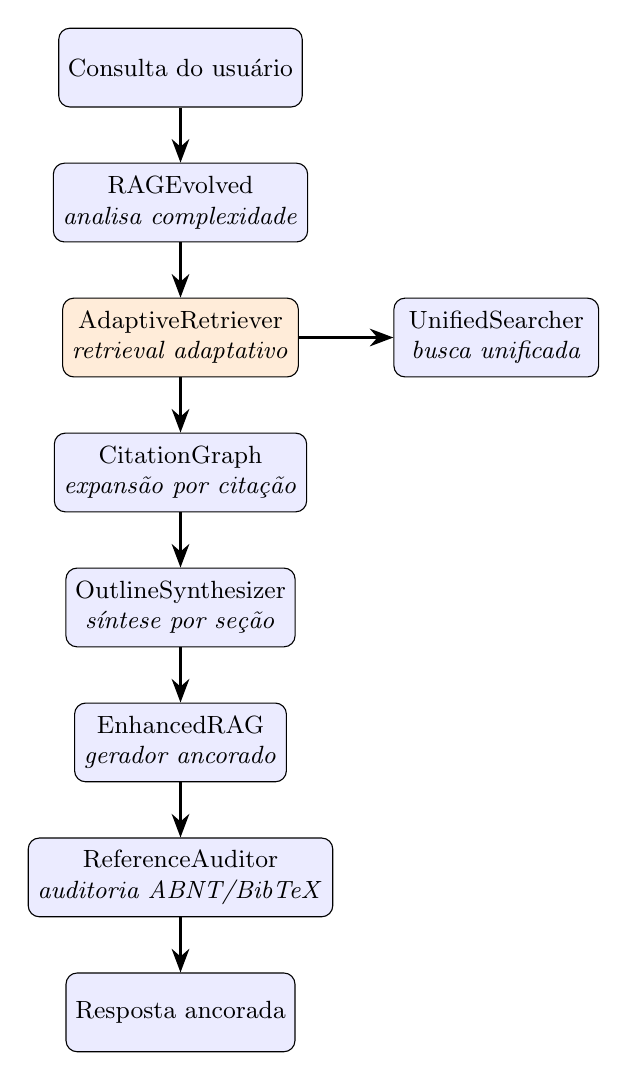
\begin{tikzpicture}[
  node distance=1.1cm,
  box/.style={draw, rounded corners, minimum width=2.6cm, minimum height=1.0cm,
              align=center, font=\small, fill=blue!8},
  arrow/.style={-{Stealth[length=3mm]}, thick}
]
  % Consulta
  \node[box] (q) {Consulta do usuário};
  \node[box, below=0.7cm of q] (ev) {RAGEvolved\\\emph{analisa complexidade}};
  \node[box, below=0.7cm of ev, fill=orange!15] (ar) {AdaptiveRetriever\\\emph{retrieval adaptativo}};
  \node[box, right=1.2cm of ar] (us) {UnifiedSearcher\\\emph{busca unificada}};
  \node[box, below=0.7cm of ar] (cg) {CitationGraph\\\emph{expansão por citação}};
  \node[box, below=0.7cm of cg] (os) {OutlineSynthesizer\\\emph{síntese por seção}};
  \node[box, below=0.7cm of os] (en) {EnhancedRAG\\\emph{gerador ancorado}};
  \node[box, below=0.7cm of en] (ra) {ReferenceAuditor\\\emph{auditoria ABNT/BibTeX}};
  \node[box, below=0.7cm of ra] (out) {Resposta ancorada};

  \draw[arrow] (q) -- (ev);
  \draw[arrow] (ev) -- (ar);
  \draw[arrow] (ar) -- (us);
  \draw[arrow] (ar) -- (cg);
  \draw[arrow] (cg) -- (os);
  \draw[arrow] (os) -- (en);
  \draw[arrow] (en) -- (ra);
  \draw[arrow] (ra) -- (out);
\end{tikzpicture}
\caption{Diagrama operacional atual do pipeline RAG. \textbf{Legenda:} caixas
azuis = componentes da recuperação/geração; caixa laranja = módulo de roteamento
adaptativo; setas = fluxo de dados. Fonte: observação do código-fonte
(\texttt{rag/evolved.py}, \texttt{rag/enhanced\_search\_rag.py}).}
\label{fig:atual}
\end{figure}

\subsection*{4.2 Insight: o roteamento adaptativo é uma heurística ponderada}

\nivel{2} Um insight que não costuma aparecer em descrições de alto nível é
\emph{como} o \texttt{AdaptiveRetriever} decide a estratégia. Observando o código,
a classificação da consulta (\texttt{simple}, \texttt{moderate}, \texttt{complex})
não é um modelo aprendido: é uma \textbf{heurística linear ponderada} sobre quatro
sinais textuais:

\begin{itemize}
  \item \textbf{Comprimento} (nº de palavras) com peso $0{,}15$;
  \item \textbf{Conceitos} (palavras capitalizadas) com peso $2{,}0$;
  \item \textbf{Conectores} lógicos/reasoning (\emph{compare}, \emph{analyze},
        \emph{synthesize}, \emph{evaluate}, \emph{implications}...) com peso $4{,}0$;
  \item \textbf{Multi-fonte} (citações autor-ano) com peso $3{,}0$.
\end{itemize}

\begin{equation}
\label{eq:complexity}
\text{score} = 0{,}15\,\text{n\_palavras} + 2\,c_{\text{conceitos}}
+ 4\,c_{\text{conectores}} + 3\,c_{\text{multi-fonte}}
\end{equation}

\noindent Consultas com $\text{score} \geq 12$ (ou com $\geq 3$ conectores em
combinação com $\geq 2$ conceitos, ou mais de 25 palavras) são tratadas como
\emph{complex}. Esse roteamento dialoga diretamente com a literatura de RAG
auto-adaptativo \cite{Jeong2024AdaptiveRAG}, mas de forma \emph{interpretável} e
determinística.

\begin{intuicao}
A heurística "conta palavras e pistas" imita como um ser humano avalia a
dificuldade: uma pergunta com "compare e analise as implicações entre A e B"
tem várias pistas de complexidade e será tratada com mais cuidado (mais
recuperação). O código torna isso explícito e reproduzível.
\end{intuicao}

\subsection*{4.3 Insight: determinismo em todos os estágios}

\nivel{2} O ecossistema demonstra uma \textbf{preocupação deliberada com
determinismo}, visível em dois pontos do código que este manual destaca pela
primeira vez:

\begin{enumerate}[label=\arabic*.]
  \item \textbf{Pontuação temporal com ano de referência fixo.} A função
        \texttt{temporal\_score} aplica \emph{decaimento exponencial} com meia-vida
        de 5 anos ($\lambda = \ln 2 / 5 \approx 0{,}1386$), mas fixa o ano de
        referência em 2026 "para determinismo em testes":
        \begin{equation}
        \label{eq:temporal}
        \text{temporal}(y) = \min\!\Bigl(0{,}07,\;
        0{,}07 \cdot e^{-0{,}1386 \cdot \max(0,\,2026-y)}\Bigr)
        \end{equation}
        Isso impede que a saída \emph{mude com a passagem do relógio}, priorizando a
        reprodutibilidade. O \textbf{clamp} em $0{,}07$ é outro insight: o bônus
        temporal é mantido \emph{pequeno e limitado}, para não virar o ranqueamento
        principal.
  \item \textbf{Expansão de consulta mínima e determinística.}
        \texttt{query\_expansion} adiciona \emph{no máximo um} sinônimo por termo
        (o primeiro em ordem alfabética) e nunca insere sinônimo já presente.
        Essa escolha evita \emph{consulta-desvio} (query drift) e garante
        reproduzibilidade, em contraste com expansões probabilísticas que poderiam
        variar entre execuções.
\end{enumerate}

\begin{pontochave}
O estado atual já incorpora determinismo como \emph{valor de engenharia}. A
proposta de Recamán estende essa filosofia ao estágio de diversificação, que hoje
é o \emph{único} ponto sem uma escolha determinística explícita.
\end{pontochave}

\subsection*{4.4 Funções dos componentes}

\nivel{1} Vamos detalhar o papel de cada componente, de forma aplicada:

\noindent\textbf{\texttt{AdaptiveRetriever}.} Analisa a complexidade da consulta
(Eq.~\ref{eq:complexity}) e escolhe entre recuperação sequencial, paralela ou
decomposta. Isso dialoga com o conceito de RAG auto-adaptativo
\cite{Jeong2024AdaptiveRAG}.

\noindent\textbf{\texttt{UnifiedSearcher}.} Agrega múltiplas fontes de busca,
deduplica resultados (por título normalizado) e aplica pontuação temporal
(Eq.~\ref{eq:temporal}). \texttt{EnhancedRAG} reutiliza a recuperação e aplica
\emph{query expansion} determinística e \emph{temporal boost}, produzindo
respostas ancoradas.

\noindent\textbf{\texttt{ReferenceAuditor}.} Normaliza títulos, formata
referências em ABNT e BibTeX, e audita consistência — alinhado ao rigor
bibliográfico do ecossistema.

\subsection*{4.5 Insight: a métrica de diversidade está ausente}

\nivel{2} Este é um dos insights mais relevantes do manual: o módulo
\texttt{EnhancedRAG.metrics()} já computa um conjunto de métricas de qualidade do
retrieval --- \emph{groundedness}, \emph{citation\_coverage},
\emph{temporal\_spread} e \emph{avg\_year} --- mas \textbf{não há nenhuma métrica
de diversidade} entre elas.

\begin{itemize}
  \item \emph{groundedness}: média dos escores de ancoragem das evidências;
  \item \emph{citation\_coverage}: fração de evidências com citação;
  \item \emph{temporal\_spread}: amplitude de anos (ano máx.\ $-$ ano mín.);
  \item \emph{avg\_year}: ano médio das evidências.
\end{itemize}

\begin{intuicao}
É como um painel de controle de um carro que mede velocidade, combustível e
temperatura --- mas não mede se os passageiros estão conversando entre si (a
"diversidade" das conversas). A proposta adiciona exatamente esse "medidor": a
métrica de diversidade (Eq.~\ref{eq:diversity}), fechando a lacuna entre o que o
sistema mede hoje e o que ele poderia medir.
\end{intuicao}

\begin{pontochave}
A lacuna de \emph{medição} de diversidade é tão importante quanto a lacuna de
\emph{implementação} de diversificação: sem métrica, não há como validar a
hipótese H1. A proposta entrega ambas.
\end{pontochave}

% =====================================================================
% SEC_05 — Proposta Pós-Recamán (Arquitetura-Alvo)
% =====================================================================

\section*{5. Proposta Pós-Recamán (Arquitetura-Alvo)}
\addcontentsline{toc}{section}{5. Proposta Pós-Recamán (Arquitetura-Alvo)}

\begin{quote}
\textbf{Aviso metodológico:} a arquitetura descrita nesta seção é uma
\textbf{proposta}, ainda \textbf{não implementada} no código-fonte. Ela representa
a arquitetura-alvo após a adoção do Diversificador de Recamán, e deve ser tratada
como desenho, não como componente observável. Em particular, nenhum dos artefatos
descritos (\texttt{ArtifactType}, \texttt{AnchorResolver},
\texttt{RecamanDiversifier}, \texttt{CanonicalContextPacker}) existe no checkout
neste momento.
\end{quote}

\subsection*{5.1 Motivação e posicionamento}

\nivel{0} Na seção anterior, vimos que o estado atual mede \emph{groundedness},
\emph{cobertura de citação} e \emph{propagação temporal}, mas \textbf{não mede nem
diversifica} o conjunto recuperado. A proposta entra exatamente nessa lacuna: um
estágio que torna a diversificação \emph{determinística} e \emph{mensurável}.

\begin{intuicao}
Voltando à analogia do bibliotecário: o sistema atual é ótimo em achar livros
\emph{relevantes} e em citá-los corretamente. A proposta acrescenta um passo
"anti-enjoo": antes de montar a mesa final, garante que os livros escolhidos
cubram ângulos distintos. E --- diferentemente de abordagens que dependem de sorte
--- esse passo é \emph{exatamente o mesmo} toda vez que a mesma pergunta é feita.
\end{intuicao}

\nivel{2} Rankeadores lexicais (BM25, Eq.~\ref{eq:bm25}) e densos tendem a
concentrar os resultados em um subespaço semântico homogêneo. Quando o objetivo é
\emph{cobrir} múltiplos ângulos de uma consulta (revisão de literatura,
sumarização, síntese multiárea), a diversidade dos candidatos é tão importante
quanto a relevância individual. A proposta introduz a diversificação
\textbf{após} o ranqueamento semântico-estrutural, usando Recamán como gerador
determinístico de \emph{offsets} --- não como substituição da relevância, mas como
mecanismo de \emph{re-balanceamento} inspirado em MMR (Eq.~\ref{eq:mmr}).

\begin{pontochave}
\emph{Posicionamento-chave:} a proposta \textbf{não compete} com o ranqueamento;
ela opera \emph{a jusante} dele, sobre a ordem já produzida. Isso garante que a
relevância primária nunca seja perdida --- apenas \emph{re-ordenada} para ganhar
cobertura.
\end{pontochave}

\subsection*{5.2 Insight: por que Recamán e não apenas randomização}

\nivel{2} Uma pergunta natural é: "por que não diversificar com uma amostragem
aleatória ou com MMR?". A resposta está na análise comparativa dos critérios:

\begin{center}
\small
\begin{tabular}{@{}L{0.14\textwidth}L{0.27\textwidth}L{0.27\textwidth}L{0.28\textwidth}@{}}
\toprule
\textbf{Critério} & \textbf{Aleatório} & \textbf{MMR} & \textbf{Recamán (proposta)} \\
\midrule
Determinismo & não & depende de $\lambda$/Sim & \textbf{sim} \\
Reprodutibilidade & baixa & parcial & \textbf{alta} \\
Custo extra & baixo & $O(K \cdot |D|)$ & \textbf{$O(K)$} \\
Sensibilidade a parâmetros & n/a & alta ($\lambda$) & \textbf{nula} \\
Interpretabilidade & baixa & média & \textbf{alta} \\
\bottomrule
\end{tabular}
\end{center}

\begin{intuicao}
Acender uma "loteria" para escolher livros funciona em média, mas não é
reproduzível (cada execução dá um resultado). O MMR é melhor, mas pede que você
defina quanto peso dar à diversidade ($\lambda$) e como medir similaridade ---
afinações que mudam o resultado. A sequência de Recamán remove essas escolhas:
dado o ranking, os offsets são \emph{fixos} e \emph{universais}. É "sorte"
determinística: sempre a mesma, mas bem distribuída.
\end{intuicao}

\subsection*{5.3 Artefatos e contratos propostos}

\nivel{1} A proposta define os seguintes artefatos (abstratos, como especificação):

\begin{itemize}
  \item \texttt{ArtifactType} --- enum que classifica o tipo de artefato
        (texto, tabela, gráfico, referência, código, dado). Este insight de design
        permite que a diversificação respeite \emph{tipos}: por exemplo, ao montar
        uma síntese, garante-se que não só textos, mas também tabelas e gráficos
        sejam representados.
  \item \texttt{AnchorResolver} --- mapeia cada artefato recuperado a uma
        \emph{âncora} canônica (citação, DOI, seção, URN interna) para ancoragem
        de diversidade. A \emph{âncora} é a chave para não contar duas versões do
        mesmo conteúdo como se fossem fontes distintas.
  \item \texttt{RecamanDiversifier} --- dado o ranking ordenado de candidatos,
        reordena/reamostra selecionando itens com \emph{offsets} derivados da
        sequência de Recamán, garantindo determinismo e reprodutibilidade.
  \item \texttt{CanonicalContextPacker} --- empacota o contexto final de forma
        canônica, respeitando a ordem de diversificação e a ancoragem.
\end{itemize}

\begin{intuicao}
A divisão em quatro artefatos segue o princípio de \emph{responsabilidade única}:
cada um faz uma coisa bem definida. \texttt{ArtifactType} "rotula" o que é;
\texttt{AnchorResolver} "amarra" cada item a uma identidade unívoca;
\texttt{RecamanDiversifier} "embaralha de forma fixa"; \texttt{ContextPacker}
"organiza a mala" final. Isso torna a proposta testável peça por peça (TDD).
\end{intuicao}

\subsection*{5.4 Insight: ancoragem canônica evita falsa diversidade}

\nivel{2} Um insight de design que merece destaque: a \emph{ancoragem canônica}
(\texttt{AnchorResolver}) resolve um problema sutil de \emph{diversidade aparente}.
Dois artefatos podem \emph{parecer} diferentes (texto distinto) mas
\emph{representar a mesma fonte} (mesmo DOI, mesma seção). Ao ancorar cada
artefato a uma identidade unívoca, a proposta evita que o diversificador
"conte duas vezes" conteúdos redundantes disfarçados de itens novos.

\begin{equation}
\label{eq:anchor}
\forall\, a \in \mathcal{S}:\; \text{âncora}(a) \in \mathcal{A},\quad
|\{\text{âncora}(a) : a \in \mathcal{S}\}| = |\mathcal{S}|
\end{equation}

\noindent A condição acima exige que todas as âncoras do conjunto selecionado
$\mathcal{S}$ sejam \emph{distintas}. Documentos que colidem na mesma âncora são
tratados como uma única fonte efetiva --- um critério essencial para que a métrica
de diversidade (Eq.~\ref{eq:diversity}) reflita \emph{diversidade real}, e não
apenas \emph{variedade de redação}.

\subsection*{5.5 Diagrama da arquitetura-alvo}

\nivel{1} O diagrama abaixo (Figura~\ref{fig:alvo}) mostra onde os novos artefatos
se encaixam, \emph{posteriores} ao ranqueamento existente.

\begin{figure}[!htb]
\centering
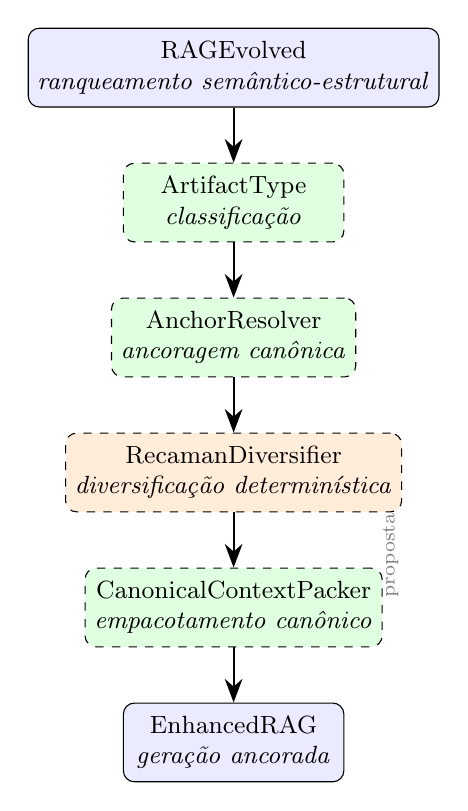
\begin{tikzpicture}[
  node distance=1.1cm,
  box/.style={draw, rounded corners, minimum width=2.8cm, minimum height=1.0cm,
              align=center, font=\small, fill=blue!8},
  prop/.style={draw, rounded corners, minimum width=2.8cm, minimum height=1.0cm,
               align=center, font=\small, fill=green!12, dashed},
  arrow/.style={-{Stealth[length=3mm]}, thick}
]
  \node[box] (ev) {RAGEvolved\\\emph{ranqueamento semântico-estrutural}};
  \node[prop, below=0.7cm of ev] (at) {ArtifactType\\\emph{classificação}};
  \node[prop, below=0.7cm of at] (ar) {AnchorResolver\\\emph{ancoragem canônica}};
  \node[prop, below=0.7cm of ar, fill=orange!15] (rd) {RecamanDiversifier\\\emph{diversificação determinística}};
  \node[prop, below=0.7cm of rd] (cp) {CanonicalContextPacker\\\emph{empacotamento canônico}};
  \node[box, below=0.7cm of cp] (en) {EnhancedRAG\\\emph{geração ancorada}};

  \draw[arrow] (ev) -- (at);
  \draw[arrow] (at) -- (ar);
  \draw[arrow] (ar) -- (rd);
  \draw[arrow] (rd) -- (cp);
  \draw[arrow] (cp) -- (en);

  \node[rotate=90, font=\scriptsize, gray, right=0.1cm of cp] {proposta};
\end{tikzpicture}
\caption{Diagrama da arquitetura-alvo pós-Recamán (proposta). \textbf{Legenda:}
caixas tracejadas verdes = novos artefatos propostos; caixa laranja tracejada =
Diversificador de Recamán (núcleo da proposta); caixas azuis sólidas = componentes
já implementados. Setas = fluxo de dados proposto. Note que a proposta \emph{se
insere} entre o ranqueamento e a geração, não substituindo nenhum componente
existente.}
\label{fig:alvo}
\end{figure}

\subsection*{5.6 Demonstração do Diversificador}

\nivel{1} Dada uma sequência ranqueada $\mathbf{r} = [r_1, r_2, \dots, r_N]$ de
candidatos e os termos da sequência de Recamán $a_0, a_1, \dots$, o diversificador
proposto seleciona candidatos percorrendo $\mathbf{r}$ com passos $a_k$, garantindo
que índices próximos (semanticamente redundantes) sejam alternados com saltos
diversificados. A Tabela~\ref{tab:offsets} ilustra os primeiros passos.

\begin{table}[!htb]
\centering
\caption{Passos derivados da sequência de Recamán para diversificação (proposta).
\textbf{Legenda:} $n$ = passo; $a_n$ = valor da sequência; exemplo de índice de
candidato selecionado sobre um ranking fictício com $N=8$.}
\label{tab:offsets}
\begin{tabular}{cccc}
\toprule
$n$ & $a_n$ & índice candidato $(1\!+\!a_n) \bmod 8$ & ilustração \\
\midrule
0 & 0 & 1 & primeiro candidato (relevância máxima) \\
1 & 1 & 2 & deslocamento de 1 posição \\
2 & 3 & 4 & salto de 3 posições (diversidade) \\
3 & 6 & 7 & salto maior \\
4 & 2 & 3 & volta a um candidato próximo \\
5 & 7 & 0 & novo salto (cobre o fim do ranking) \\
\bottomrule
\end{tabular}
\end{table}

\nivel{2} A Tabela~\ref{tab:offsets} evidencia a \emph{alternância} entre saltos
curtos e longos, característica da sequência de Recamán. Esse padrão é um insight
crucial: ao alternar $a_n$ entre valores pequenos e grandes, o diversificador
"varre" tanto as regiões de alta relevância (início do ranking) quanto as de maior
cobertura (final), cobrindo \emph{simultaneamente} relevância e diversidade --- em
linha com o espírito do MMR, mas sem parâmetros $\lambda$.

\begin{pontochave}
Em uma frase: \emph{o MMR equilibra relevância e novidade usando um parâmetro; a
proposta equilibra usando a própria geometria da sequência de Recamán ---
deterministicamente.}
\end{pontochave}

% =====================================================================
% SEC_06 — Cálculos e Especificações Técnicas
% =====================================================================

\section*{6. Cálculos e Especificações Técnicas}
\addcontentsline{toc}{section}{6. Cálculos e Especificações Técnicas}

\nivel{0} Esta seção transforma as ideias das seções anteriores em números e
contratos precisos: como \emph{medir} diversidade, quanto \emph{custa} a proposta
e o que \emph{muda} (antes/depois) na especificação. É aqui que a proposta sai do
"discurso" e vira \emph{especificação verificável}.

\subsection*{6.1 Métricas de diversidade}

\nivel{2} Sobre um conjunto de candidatos selecionados $\mathcal{S}$, definimos a
diversidade média entre os itens recuperados:

\begin{equation}
\label{eq:diversity}
\text{Div}(\mathcal{S})\;=\;\frac{1}{|\mathcal{S}|(|\mathcal{S}|-1)}
\sum_{\substack{i \neq j \\ r_i, r_j \in \mathcal{S}}}
\bigl(1 - \text{Sim}(r_i, r_j)\bigr)
\end{equation}

\noindent onde $\text{Sim}(\cdot,\cdot) \in [0,1]$ é uma medida de similaridade
normalizada (coseno ou Jaccard sobre âncoras). Valores de $\text{Div}(\mathcal{S})$
próximos de $1$ indicam alta diversidade; valores próximos de $0$ indicam
redundância.

\begin{intuicao}
A fórmula apenas computa, em média, "o quanto os itens são diferentes entre si".
Se todos os livros falam do mesmo assunto (similaridade $1$), a diversidade é $0$.
Se cada um é disjunto (similaridade $0$), a diversidade é $1$. Simples e poderoso.
\end{intuicao}

\nivel{2} \textbf{Insight de rigor: a escolha do $\text{Sim}$ importa.} Se a
similaridade for medida sobre \emph{texto bruto} (coseno de embeddings), dois
textos com redação distinta mas mesma fonte terão $\text{Sim}$ baixo e a métrica
superestimará a diversidade. Por isso a proposta vincula a métrica às
\emph{âncoras canônicas} (Eq.~\ref{eq:anchor}): ao computar a similaridade sobre
identidade de fonte/âmago, a $\text{Div}$ reflete \emph{diversidade efetiva}
(conteúdo realmente distinto), não \emph{variedade de redação}. Essa é uma decisão
metodológica explícita e verificável.

\subsection*{6.2 Custo computacional do Diversificador}

\nivel{2} A sequência de Recamán até o passo $M$ pode ser gerada em $O(M)$ de
tempo com memória $O(M)$ (mantendo o conjunto dos valores já visitados). Para um
ranking de $N$ candidatos e um orçamento de $K$ seleções, o Diversificador
proposto opera, no pior caso, em $O(K)$ sobre o ranking indexado, com memória
adicional $O(N)$ para as âncoras e $O(N)$ para o conjunto de valores da sequência.

\begin{intuicao}
"Custo $O(K)$" significa: o esforço cresce \emph{linearmente} com quantos itens
queremos selecionar. Se dobrar a quantidade de seleções, dobra o esforço --- nada
de explosão. Comparado com a \emph{codificação de embeddings} dos documentos
(tipicamente o gargalo), o diversificador é negligível.
\end{intuicao}

\nivel{2} \textbf{Análise de rigor:} decompomos o custo em dois termos:

\begin{equation}
\label{eq:cost}
T(N,K) \;=\; \underbrace{O(K)}_{\text{seleção via offsets}}
\;+\; \underbrace{O(N)}_{\text{geração/consulta de âncoras}}
\end{equation}

\noindent O primeiro termo ($O(K)$) cobre o percurso do ranking com os offsets de
Recamán; o segundo ($O(N)$) cobre a resolução de âncoras para classificar e deduplicar
os $N$ candidatos disponíveis. Como, na prática, $K \leq N$, o custo total é
dominado por $O(N)$ --- assintoticamente o mesmo custo de \emph{ler} os candidatos,
ou seja, \textbf{não adiciona um termo dominante novo} ao pipeline. Isso contrasta
com o MMR, cuja etapa de seleção pode atingir $O(K \cdot |D|)$ por causa da
comparação $\max_{d_j \in D} \text{Sim}_2(d,d_j)$ (Eq.~\ref{eq:mmr}).

\begin{pontochave}
\begin{tabularx}{\textwidth}{lXX}
\toprule
\textbf{Estágio} & \textbf{Complexidade} & \textbf{Observação} \\
\midrule
Geração de Recamán ($M$ termos) & $O(M)$ tempo, $O(M)$ memóri & valores visitados em \texttt{set} \\
Seleção de $K$ itens & $O(K)$ & percurso com offsets \\
Resolução de âncoras & $O(N)$ & deduplicação por identidade \\
\textbf{Total} & $O(N)$ & não domina o pipeline \\
\bottomrule
\end{tabularx}
\end{pontochave}

\subsection*{6.3 Insight: conexão com o efeito "perdido no meio"}

\nivel{2} Um insight que conecta a proposta à literatura de forma não trivial: o
efeito \emph{lost in the middle} \cite{Liu2024LostMiddle} mostra que modelos de
linguagem têm desempenho assimétrico em relação à posição dos documentos no
contexto longo (tendem a "esquecer" o que está no meio). A \emph{ordem} em que o
contexto é montado --- e que o \texttt{CanonicalContextPacker} define --- não é um
detalhe cosmético: ela afeta diretamente a qualidade da geração.

\begin{equation}
\label{eq:positional}
\Pr[\text{documento } r \text{ ser usado}] \;\approx\;
g\bigl(\text{posição}(r)\bigr),\quad
g \text{ não monótona (efeito em U)}
\end{equation}

\noindent A literatura sugere um efeito em forma de \emph{U}: início e fim do
contexto são mais bem utilizados do que o meio \cite{Liu2024LostMiddle}. Isso
confere \emph{relevância funcional} à proposta: não basta selecionar documentos
diversos; é preciso \emph{posicioná-los} de forma canônica no contexto para
maximizar a chance de uso. O \texttt{CanonicalContextPacker} torna esse
posicionamento \emph{determinístico} e \emph{auditável}, uma dimensão que o
estado atual não formaliza.

\begin{intuicao}
Se o gerador "presta menos atenção" no meio do texto, ao montar o contexto
devemos ser espertos sobre a ordem: colocar os documentos mais importantes no
início e no fim. O \emph{empacotador canônico} garante que essa ordem seja sempre
a mesma, tornando o comportamento previsível e testável.
\end{intuicao}

\subsection*{6.4 Insight: três dimensões ortogonais de qualidade}

\nivel{2} Consolidando as seções precedentes, o estado atual já mede duas
dimensões de qualidade do retrieval (\emph{groundedness} e
\emph{citation\_coverage}), além de \emph{temporal\_spread}. A proposta adiciona
uma terceira e distinta dimensão --- \emph{diversidade}:

\begin{itemize}
  \item \textbf{groundedness} --- quão ancoradas estão as evidências;
  \item \textbf{citation\_coverage} --- quão bem citadas;
  \item \textbf{diversity} (nova) --- quão \emph{cobertos} estão os ângulos.
\end{itemize}

\noindent A ortogonalidade dessas dimensões é o que permite avaliar a hipótese H1
sem ambiguidade: um sistema pode ter \emph{alta} groundedness e \emph{alta}
diversidade simultaneamente --- não são métricas concorrentes. O painel de
controle do \texttt{EnhancedRAG.metrics()} passa, na arquitetura-alvo, a incluir
$\text{Div}(\mathcal{S})$ como quinto campo (Eq.~\ref{eq:diversity}), fechando a
lacuna de medição identificada na Seção~4.

\subsection*{6.5 Antes/depois: contrato da especificação}

\nivel{1} A Tabela~\ref{tab:spec} resume as especificações técnicas do estado atual
e da arquitetura-alvo proposta.

\begin{table}[!htb]
\centering
\caption{Especificações técnicas comparadas: estado atual vs.\ proposta
pós-Recamán. \textbf{Legenda:} CH = implementado no checkout; PROP = proposta não
implementada.}
\label{tab:spec}
\begin{tabularx}{\textwidth}{lXX}
\toprule
\textbf{Aspecto} & \textbf{Estado atual} & \textbf{Proposta (pós-Recamán)} \\
\midrule
Ranqueamento primário & BM25/denso (Eq.~\ref{eq:bm25}) & preservado, sem alteração \\
Roteamento adaptativo & \texttt{AdaptiveRetriever} (CH) & preservado \\
Diversificação & via MMR conceitual & \texttt{RecamanDiversifier} (PROP) \\
Classificação de artefato & ausente & \texttt{ArtifactType} (PROP) \\
Ancoragem canônica & parcial (auditoria) & \texttt{AnchorResolver} (PROP) \\
Empacotamento & \texttt{CanonicalContextPacker} (PROP) & proposto \\
Reprodutibilidade da diversif. & não determinística & determinística (Recamán) \\
Métrica de diversidade & ausente & $\text{Div}(\mathcal{S})$ (Eq.~\ref{eq:diversity}) \\
Custo assimptótico extra & n/a & $O(N)$ (Eq.~\ref{eq:cost}) \\
\bottomrule
\end{tabularx}
\end{table}

\begin{pontochave}
A especificação evolui de forma \emph{aditiva}: nada do que existe hoje é
removido ou alterado em contrato público. A proposta \emph{insere} novos
componentes e uma nova métrica, respeitando o princípio de compatibilidade
retrógrada dos fluxos consumidores.
\end{pontochave}

% =====================================================================
% SEC_07 — Implementações Reproduzíveis
% =====================================================================

\section*{7. Implementações Reproduzíveis}
\addcontentsline{toc}{section}{7. Implementações Reproduzíveis}

\nivel{0} Toda o arcabouço teórico das seções anteriores precisa, em última
instância, se materializar em \emph{código executável e reproduzível}. Esta seção
percorre, em ordem didática, os três alicerces práticos: (1) \emph{o quê} gera a
sequência determinística; (2) \emph{como} o diversificador a consome; e (3)
\emph{com que ferramenta} tudo isso é compilado e auditado. A lógica segue a do
ecossistema: \emph{testes primeiro} (RED), \emph{implementação} (GREEN) e
\emph{refatoração} (REFACTOR), dentro do protocolo TDD.

\subsection*{7.1 Geração determinística da sequência de Recamán}

\nivel{1} O Algoritmo~\ref{alg:recaman} gera os primeiros $M$ termos da sequência
de Recamán (Eq.~\ref{eq:recaman}). Sua execução é totalmente reprodutível: para o
mesmo $M$, a saída é bit a bit idêntica em qualquer ambiente.

\begin{algorithm}[!htb]
\caption{Geração determinística da sequência de Recamán}
\label{alg:recaman}
\begin{algorithmic}[1]
\Require $M \geq 1$ (número de termos desejado), com $a_0 = 0$
\Ensure $a[0..M]$ tais que satisfaçam a Eq.~\ref{eq:recaman}
\State $a[0] \gets 0$
\State $\text{seen} \gets \{0\}$
\For{$n \gets 1$ \textbf{to} $M$}
  \State $\text{cand} \gets a[n-1] - n$
  \If{$\text{cand} > 0$ \textbf{and} $\text{cand} \notin \text{seen}$}
    \State $a[n] \gets \text{cand}$
  \Else
    \State $a[n] \gets a[n-1] + n$
  \EndIf
  \State $\text{seen} \gets \text{seen} \cup \{a[n]\}$
\EndFor
\State \Return $a$
\end{algorithmic}
\end{algorithm}

\nivel{2} \textbf{Insight de implementação: a garantia de determinismo}. A
reprodutibilidade vem de três detalhes que, isoladamente, podem parecer triviais,
mas juntos asseguram a invariância:

\begin{enumerate}[label=\arabic*.]
  \item \emph{Ordem determinística de avaliação} --- a condição testa primeiro
        $a_{n-1} - n > 0$ e, só então, a pertinência a \texttt{seen}; essa ordem
        é fixa e documentada.
  \item \emph{Conjunto de visitados} (\texttt{seen}) --- implementável como um
        \texttt{set} (hash) ou uma \texttt{bitset}; o conteúdo (não a ordem
        interna) é o que importa para decidir a pertinência.
  \item \emph{Independência de \emph{seed}} --- ao contrário de amostragens
        aleatórias, não há gerador pseudoaleatório, logo não há \emph{seed} que
        altere o resultado.
\end{enumerate}

\begin{intuicao}
O algoritmo é "uma receita de bolo com medidas exatas": não importa quem execute
nem em que máquina --- o bolo (a sequência) sai idêntico. Isso permite que testes
automáticos (TDD) verifiquem valores esperados conhecidos da sequência, como
$a_0 = 0$, $a_1 = 1$, $a_2 = 3$, $a_3 = 6$, $a_4 = 2$, $a_5 = 7$.
\end{intuicao}

\begin{pontochave}
Os primeiros termos conhecidos (OEIS A005132) $0,1,3,6,2,7,13,\dots$ servem como
\emph{oráculo de teste}: um teste TDD pode afirmar que
\texttt{recaman\_sequence(6) == [0,1,3,6,2,7]}, transformando a reprodutibilidade
em algo \emph{verificável por máquina}.
\end{pontochave}

\subsection*{7.2 Esboço da interface do Diversificador}

\nivel{1} O trecho abaixo esquematiza a interface proposta (não implementada) do
\texttt{RecamanDiversifier}. Ele consome o ranking e os offsets da sequência para
selecionar $k$ candidatos.

\begin{lstlisting}[language=Python, caption={Esboço de interface do RecamanDiversifier (proposta, não implementada).}]
class RecamanDiversifier:
    """Deterministic diversifier based on the Recaman sequence.

    PROPOSAL - NOT implemented in the checkout.
    """
    def __init__(self, seen=None):
        self.a = [0]
        self.seen = seen or {0}

    def next_offset(self, n):
        # generates a_n per the Recaman Eq. (O(1) amortized)
        prev = self.a[n - 1]
        cand = prev - n
        if cand > 0 and cand not in self.seen:
            val = cand
        else:
            val = prev + n
        self.a.append(val)
        self.seen.add(val)
        return val

    def diversify(self, ranked, k):
        """Selects k candidates from 'ranked' using Recaman offsets."""
        selected = []
        cursor = 0
        n = 0
        while len(selected) < k and cursor < len(ranked):
            selected.append(ranked[cursor])
            offset = self.next_offset(n)
            cursor = (cursor + offset + 1) % len(ranked)
            n += 1
        return selected
\end{lstlisting}

\nivel{2} \textbf{Insight de desenho: `next\_offset` é o coração reutilizável.} O
método \texttt{next\_offset(n)} isola a \emph{geração incremental} da sequência,
separando-a da \emph{lógica de seleção} (\texttt{diversify}). Essa separação é
didática e de engenharia: permite testar a geração de offsets isoladamente
(propriedades de Recamán) e a seleção separadamente (cobertura do ranking).

\begin{intuicao}
Separar "gerar o número do salto" de "decidir para onde saltar" é como separar a
fábrica de "chaves" da fechadura que as usa: cada parte pode ser testada e
ajustada sem quebrar a outra.
\end{intuicao}

\nivel{2} \textbf{Insight de correção: a estrutura do laço garante terminação.} O
laço de \texttt{diversify} avança o cursor com \texttt{(cursor + offset + 1) \% len(ranked)}.
Ao usar o módulo, o cursor permanece sempre no intervalo $[0, N-1]$, e a condição
\texttt{len(selected) < k} limita o total de iterações a, no máximo, $k$ ---
garantindo terminação e um limite superior de $O(k)$ operações (consistente com a
Eq.~\ref{eq:cost}).

\begin{pontochave}
Ética de implementação: o esboço é \emph{legível} e \emph{testável} por partes.
Antes de qualquer uso em produção, ele deve passar por um ciclo TDD completo:
testar determinismo (mesma entrada, mesma saída), testar cobertura e testar a
terminação para todos os $N$ e $k$ de interesse.
\end{pontochave}

\subsection*{7.3 Compilação do manual}

\nivel{1} O PDF deste manual é compilado de forma reproduzível com os comandos:

\begin{lstlisting}[language=bash, caption={Comando de compilação reproduzível do manual.}]
cd docs/r456_manual_tecnico_rag
./build.sh            # uses pdflatex + bibtex + makeindex
# or, alternatively:
make                  # uses latexmk -pdf
\end{lstlisting}

\nivel{2} A toolchain exigida é TeX Live com \texttt{pdflatex}, \texttt{bibtex},
\texttt{makeindex} e \texttt{latexmk}, e a classe local \texttt{abntex2} do
diretório \texttt{publishing/templates/abntex2}. Para que a compilação encontre a
classe e os estilos bibliográficos \emph{copiados no repositório} (e não os do
sistema), é necessário expor três variáveis de ambiente:

\begin{lstlisting}[language=bash, caption={Variáveis de ambiente para localizar a classe abntex2 local.}]
export TEXINPUTS=".:../../publishing/templates/abntex2/:${TEXINPUTS}"
export BSTINPUTS=".:../../publishing/templates/abntex2/:${BSTINPUTS}"
export BIBINPUTS=".:../../publishing/templates/abntex2/:${BIBINPUTS}"
\end{lstlisting}

\begin{intuicao}
Pense nessas variáveis como o "caminho até a biblioteca": o \LaTeX{} precisa saber
onde estão as classes e estilos que você não instalou globalmente. Apontando para
a pasta do repositório, garantimos que a mesma versão da classe seja usada em
qualquer máquina --- mais uma camada de reprodutibilidade.
\end{intuicao}

\begin{pontochave}
A reprodutibilidade não se limita ao \emph{código do diversificador}: ela se
estende à \emph{geração deste próprio manual}. O mesmo princípio de "saída
idêntica para a mesma entrada" guia a compilação via \texttt{build.sh}/\texttt{make}.
\end{pontochave}

% =====================================================================
% SEC_08 — Mapas de Dados e Diagrama Operacional
% =====================================================================

\section*{8. Mapas de Dados e Diagrama Operacional}
\addcontentsline{toc}{section}{8. Mapas de Dados e Diagrama Operacional}

\nivel{0} Até aqui vimos os conceitos (Seção 3), o que existe (Seção 4), a
proposta (Seção 5), as métricas (Seção 6) e o código (Seção 7). Falta uma camada
"cartográfica": como a proposta se encaixa no \emph{mapa geral} do ecossistema e
em quais fluxos ela tem efeito. Esta seção desenha o "mapa do território".

\subsection*{8.1 O papel dos mapas de dados no ecossistema}

\nivel{1} O ecossistema mantém mapas de dados e mapas de arquitetura em
\texttt{docs/} (por exemplo, \texttt{MAPA\_ARQUITETURA\_R433\_R438.md},
\texttt{architecture\_map.html}). Estes artefatos documentais informam tanto o
estado atual quanto o desenho da proposta, preservando a riqueza dos fluxos
multiárea: acadêmico, formal, jurídico, clínico, MIRA, RAG, Universidade
Sintética, runtimes locais e gates de qualidade/integridade.

\begin{intuicao}
Um mapa de arquitetura é como o mapa de um metrô: não mostra cada trilho, mas
mostra as \emph{linhas} (fluxos) e as \emph{estações} (subsistemas) e como elas
se conectam. O RAG é uma das "linhas" que cruza várias outras.
\end{intuicao}

\subsection*{8.2 Insight: o RAG como subsistema transversal}

\nivel{2} Um insight estrutural que o mapa revela é que o RAG \emph{não pertence a
um único fluxo}: ele é um subsistema \emph{transversal}, reutilizado por múltiplos
fluxos. A Figura~\ref{fig:transversal} ilustra essa transversalidade de forma
conceitual.

\begin{figure}[!htb]
\centering
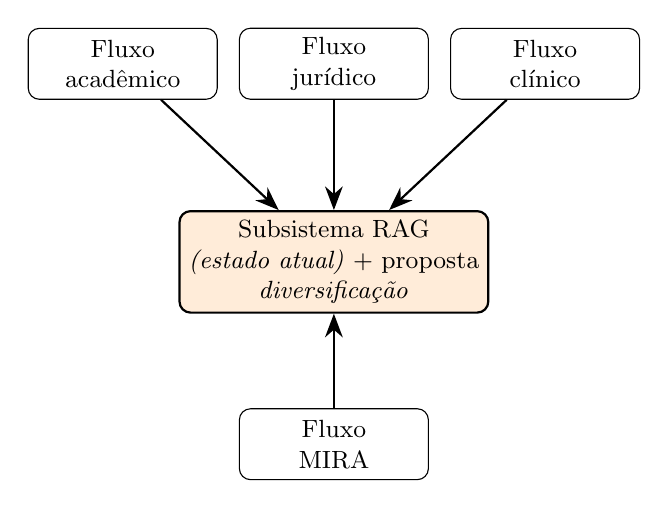
\begin{tikzpicture}[
  node distance=1.0cm,
  flujo/.style={draw, rounded corners, minimum width=2.4cm, minimum height=0.9cm,
                align=center, font=\small},
  ragbox/.style={draw, rounded corners, minimum width=2.6cm, minimum height=1.1cm,
                 align=center, font=\small, fill=orange!15, thick},
  arrow/.style={-{Stealth[length=3mm]}, thick}
]
  \node[ragbox] (rag) {Subsistema RAG\\\emph{(estado atual)} + proposta\\\emph{diversificação}};
  \node[flujo, above left=1.4cm and -0.5cm of rag] (ac) {Fluxo\\acadêmico};
  \node[flujo, above=1.4cm of rag] (ju) {Fluxo\\jurídico};
  \node[flujo, above right=1.4cm and -0.5cm of rag] (cl) {Fluxo\\clínico};
  \node[flujo, below=1.2cm of rag] (mi) {Fluxo\\MIRA};

  \draw[arrow] (ac) -- (rag);
  \draw[arrow] (ju) -- (rag);
  \draw[arrow] (cl) -- (rag);
  \draw[arrow] (mi) -- (rag);
\end{tikzpicture}
\caption{Transversalidade conceitual do subsistema RAG. \textbf{Legenda:} caixa
laranja = subsistema RAG (estado atual) com a proposta de diversificação; caixas
azuis = fluxos consumidores. As setas indicam dependência dos fluxos em relação ao
RAG. A diversificação proposta atua \emph{no interior} do subsistema, sem alterar a
interface pública dos fluxos e sem exigir mudança neles.}
\label{fig:transversal}
\end{figure}

\nivel{2} \textbf{Por que isso é relevante para a proposta:} como o RAG é
transversal, qualquer melhoria interna --- como a diversificação por Recamán ---
propaga-se \emph{sem custo de integração} para todos os fluxos dependentes. Isso
explica a RQ4 (impacto multiárea): o ganho potencial não exige tocar em cada fluxo
individualmente; basta melhorar o subsistema compartilhado.

\begin{pontochave}
A transversalidade é um \emph{multiplicador de impacto}: uma melhoria única no
subsistema RAG beneficia os fluxos acadêmico, jurídico, clínico e MIRA
simultaneamente, com o mesmo esforço de implementação.
\end{pontochave}

\subsection*{8.3 Integração do RAG nos fluxos multiárea}

\nivel{1} Concretizando: o RAG atua como subsistema transversal e serve ao fluxo
acadêmico (revisão de literatura), ao fluxo jurídico (recuperação normativa), ao
fluxo clínico (suporte à decisão) e ao fluxo MIRA (geração de conteúdo). A proposta
de diversificação por Recamán visa melhorar a \emph{cobertura semântica} desse
subsistema transversal, sem alterar a interface pública dos fluxos consumidores.

\nivel{2} \textbf{Insight de rigor: "sem alterar a interface" é um contrato, não
uma promessa.} Preservar a interface pública dos fluxos é um critério de desenho
\textbf{verificável}: os fluxos continuam a consumir as mesmas entradas/saídas do
subsistema RAG. A diversificação ocorre \emph{internamente}, no conjunto de
candidatos selecionados antes da geração, de modo que a assinatura de chamada e o
formato de resposta permanecem compatíveis. Esse é um requisito que será
verificado por testes de regressão de interface no trabalho futuro.

\begin{pontochave}
O mapa mostra que a proposta é \emph{adicional} e \emph{localizada}: ela enriquece
o subsistema transversal mantendo o restante do território intacto. É uma
mudança de \emph{alto impacto, baixo risco de integração}.
\end{pontochave}

% =====================================================================
% SEC_09 — Considerações Finais e Trabalho Futuro
% =====================================================================

\section*{9. Considerações Finais e Trabalho Futuro}
\addcontentsline{toc}{section}{9. Considerações Finais e Trabalho Futuro}

\nivel{0} Chegamos ao fim. Esta seção amarra o fio narrativo: retomamos o problema
de pesquisa da Seção~2, verificamos como cada seção contribuiu para resolvê-lo e
definimos um \emph{roadmap concreto} de trabalho futuro, com etapas verificáveis e
métricas de aceitação. Nada de promessas vagas: cada item tem critério e
responsável (o protocolo TDD do ecossistema).

\subsection*{9.1 Síntese: o caminho percorrido}

\nivel{1} O manual seguiu uma sequência lógica que pode ser resumida em um único
fluxo de raciocínio:

\begin{center}
\begin{tabularx}{\textwidth}{lX}
\toprule
\textbf{Etapa} & \textbf{O que se estabeleceu} \\
\midrule
Seção 1 & Leitor é orientado sobre como ler (trilha N0--N2). \\
Seção 2 & Problema de pesquisa (PP), 4 RQs e hipótese H1 são formalizados. \\
Seção 3 & Base teórica: BM25, RAG, raciocínio, MMR e Recamán. \\
Seção 4 & Estado atual: pipeline implementado e \emph{lacuna} de diversidade. \\
Seção 5 & Proposta pós-Recamán: 4 artefatos e posicionamento aditivo. \\
Seção 6 & Cálculos: métricas, custo $O(N)$ e conexão com "lost in the middle". \\
Seção 7 & Implementações: algoritmo, interface e reprodutibilidade. \\
Seção 8 & Mapas: transversalidade e impacto sem quebrar interfaces. \\
\bottomrule
\end{tabularx}
\end{center}

\begin{pontochave}
O fio condutor único: \emph{um problema real} (concentração de resultados)
$\rightarrow$ \emph{uma hipótese} (diversificação determinística via Recamán)
$\rightarrow$ \emph{uma especificação} (artefatos + métricas) $\rightarrow$ \emph{uma
implementação reproduzível}.
\end{pontochave}

\subsection*{9.2 Retomada do problema e das hipóteses}

\nivel{2} Voltando à Seção~2: o problema de pesquisa (PP) pedia uma diversificação
estruturada determinística, pós-ranqueamento, com custo controlado. O manual
\emph{responde} a cada componente:

\begin{itemize}
  \item \textbf{Determinismo} --- respondido pela sequência de Recamán
        (Eq.~\ref{eq:recaman}), que é uma função matemática canônica, sem
        \emph{seed} (Seções 5 e 7).
  \item \textbf{Pós-ranqueamento} --- o \texttt{RecamanDiversifier} opera sobre o
        ranking já ordenado, sem alterar o ranqueador (Seção 5).
  \item \textbf{Custo controlado} --- demonstrado em $O(N)$ (Eq.~\ref{eq:cost}),
        não dominante no pipeline (Seção 6).
\end{itemize}

\noindent A hipótese H1, portanto, permanece \textbf{plausível e mensurável}, mas
\textbf{não verificada}: sua confirmação exige implementação e experimentação
empírica. Este manual a \emph{formula} e a \emph{prepara}, sem a \emph{provar}.

\subsection*{9.3 Roadmap de trabalho futuro (concreto e verificável)}

\nivel{1} Definimos um roadmap em fases, cada uma com \textbf{critério de aceitação
mensurável} e alinhado às RQs. Este é o plano \emph{ação-ação}, passível de virar
specs SDD/TDD:

\begin{enumerate}[label=\textbf{Fase \arabic*.}]
  \item \textbf{Implementação do \texttt{RecamanDiversifier}} (RQ2, RQ3).
        \begin{itemize}
          \item \emph{Ação:} criar \texttt{rag/recaman.py} com a interface da
                Seção~7, seguindo TDD (RED$\to$GREEN$\to$REFACTOR).
          \item \emph{Critério:} testes deterministas ($a_0\!..\!a_5 =
                [0,1,3,6,2,7]$), terminação para todos os $N$,$k$, e
                $\text{Div}(\mathcal{S})$ mensurável.
        \end{itemize}
  \item \textbf{Métrica de diversidade no \texttt{EnhancedRAG.metrics()}} (RQ1).
        \begin{itemize}
          \item \emph{Ação:} adicionar o campo $\text{Div}(\mathcal{S})$
                (Eq.~\ref{eq:diversity}) ao painel de métricas existente, ligado a
                \texttt{AnchorResolver}.
          \item \emph{Critério:} painel passa a reportar diversidade; teste
                garante $\text{Div}\in[0,1]$ e coerência com \emph{groundedness}.
        \end{itemize}
  \item \textbf{Experimento de coorte em corpus-piloto} (RQ1, RQ4).
        \begin{itemize}
          \item \emph{Ação:} comparar diversidade e groundedness entre estado
                atual, MMR e Recamán em um corpus real do ecossistema.
          \item \emph{Critério:} relatório com $\text{Div}$, groundedness e
                \emph{baseline} justo (mesmos dados, mesmas seeds, mesmo oráculo).
        \end{itemize}
  \item \textbf{Teste de regressão de interface} (RQ4).
        \begin{itemize}
          \item \emph{Ação:} garantir que fluxos (acadêmico, jurídico, clínico,
                MIRA) continuem consumindo o RAG sem mudança de contrato.
          \item \emph{Critério:} suíte de regressão verde sobre a interface pública
                dos fluxos.
        \end{itemize}
  \item \textbf{Registro evolutivo} (governança).
        \begin{itemize}
          \item \emph{Ação:} registrar cada ciclo no \texttt{evolution/cycles.json}
                e no MetaBus, conforme o protocolo do ecossistema.
          \item \emph{Critério:} ciclo R456+ registrado com score e lições;
                MetaBus acessível.
        \end{itemize}
\end{enumerate}

\begin{intuicao}
O roadmap é como a "lista de tarefas de um projeto": cada linha tem um \emph{o
que fazer} (ação), um \emph{como saber que deu certo} (critério) e uma \emph{ligação
com a pergunta de pesquisa} (RQ). Isso transforma intenções em trabalho auditável.
\end{intuicao}

\subsection*{9.4 Contribuições esperadas (com rigor)}

\nivel{2} As contribuições esperadas deste trabalho, de forma \emph{cautelosa} e
sem \emph{overclaim}, são:

\begin{enumerate}[label=\arabic*.]
  \item \textbf{Contribuição metodológica:} uma ponte determinística entre teoria
        dos números (Recamán) e diversificação de recuperação, oferecendo um
        \emph{baseline reproduzível} e comparável (Seções 5--6).
  \item \textbf{Contribuição de engenharia:} uma especificação aditiva e de baixo
        acoplamento para o ecossistema, com custo $O(N)$ e preservação de
        interface (Seções 6 e 8).
  \item \textbf{Contribuição de medição:} o fechamento da lacuna de \emph{métrica de
        diversidade} do painel atual (Seção 4), permitindo avaliar a hipótese H1.
\end{enumerate}

\begin{pontochave}
Diferentemente de relatos que superestimam resultados, este manual declara
\emph{contribuições esperadas} e \emph{hipotéticas}, vinculadas a RQs e métricas
— nunca como fatos consumados.
\end{pontochave}

\subsection*{9.5 Considerações éticas e de rigor final}

\nivel{2} Reafirmamos os compromissos éticos e de rigor que atravessaram todo o
documento:

\begin{itemize}
  \item \textbf{Anti-overclaim:} nenhuma certificação externa, segurança absoluta
        ou disponibilidade universal é alegada.
  \item \textbf{Transparência:} estado atual e proposta estão separados e
        rotulados; nenhum componente proposto é apresentado como implementado.
  \item \textbf{Mensurabilidade:} todo impacto potencial está vinculado a uma RQ e
        a uma métrica (Eq.~\ref{eq:diversity}), a ser validada empiricamente.
  \item \textbf{Reprodutibilidade:} algoritmos, métricas e até a compilação deste
        manual são reproduzíveis (Seção 7).
\end{itemize}

\begin{pontochave}
O fecho deste manual não é um ponto final, mas um \emph{ponto de partida}:
deixamos o problema formulado, a hipótese preparada e o roadmap aberto, prontos
para migrar da \emph{especificação} para a \emph{implementação verificável}.
\end{pontochave}


% ---------------------------------------------------------------------
% Referências (unificadas de todo o documento)
% ---------------------------------------------------------------------
\clearpage
\bibliography{referencias}
\bibliographystyle{abntex2-alf}

\end{document}
